\documentclass[12pt]{article}
\usepackage[spanish, es-tabla]{babel}
\usepackage{amssymb, amsmath}
\usepackage{float}
\usepackage{graphicx}
\usepackage[export]{adjustbox}
\title{Matemáticas para las Ciencias Aplicadas \\ Tarea 1}
\date{}
\author{Garcia Islas Fernando \\ Leo\\Mariana}
\begin{document}
\maketitle
\section{\large Un cohete}
Un cohete es disparado verticalmente hacia arriba y el combustible que lo impulsa se quema durante 60 segundos. Se sabe que, a los $h$ s de haber iniciado su desplazamiento, la altura $h$ (en metros) a la que se encuentra el cohete es: \[h(t) = 40 t^2 \; m\]
\begin{enumerate}

%Punto 1 del ejercicio 1
\item ¿A qué altura se halla el cohete cuando se le agota el combustible?
  
  \begin{align*}
    h(t)= 40t^2 \; \text{m} \hspace{5.1cm}    h(t)&=40(60)^2 \; m\\
t=60\text{s} \hspace{7cm}    &=40(3600) \; m\\
    &=144,000 \; m\\
  \end{align*}
  
  {\bf R:} 144,000 m es la altura cuando se agota el combustible.
  
  %Punto 2 del ejercicio 1
\item ¿Cuál es la rapidez promedio del cohete durante los primeros 60 s de su vuelo?
  
  \begin{align*}
    &\text{Rapidez promedio}=\frac{d}{t} \hspace{3cm}\frac{144,000}{60}= 2400 \frac{m}{s}\\
    &t = 60\; \text{s} \\
    &d = 40t^2 \; \text{m} 
  \end{align*}
  
  {\bf R:} $2,400 \frac{m}{s}$ es la rapidez promedio.
  
  %Punto 3 del ejercicio 1
\item Haga una tabla con tres columnas: una para el tiempo $t$ (donde $t = 0, 10, 20, . . . , 60 $s); otra para la posición $h(t)$; y una tercera para el incremento $\Delta h$ entre un valor de $t$ y el siguiente. Con base en ella, calcule la rapidez promedio del cohete para cada lapso de 10 s desde $t = 0$ hasta $t = 60$.
  
  \begin{table}[h]
  
    \begin{center}
  
        \begin{tabular}{| c | c | c |c|}\hline %Tabla 1
            $\Delta t$ s & $h(t)$ m & $\Delta h$ m&$\frac{h(t)}{t}\frac{m}{s}$\\ \hline
            0 & 0 & 0 &0 \\ 
            10& 4000& 4000& 4000 \\
            20&16,000&12,000&800\\
            30&36,000&20,000&1,200\\
            40&64,000&28,000&1,600\\
            50&100,000&36.000&2,000\\
            60& 144,000& 44,000& 2,400 \\ \hline
        \end{tabular}
    
    \caption{Rapidez promedio de intervalos $\Delta t$} 
    
    \label{tab:rapprom}
    
    \end{center}
  
  \end{table}

%Punto 4 del ejercicio 1
\item Haga ahora otra tabla en la que muestre el cálculo de la rapidez promedio del cohete $\Delta t$ s antes y $\Delta t$ s después de $t = 3$ s, para los siguientes valores de $\Delta t$:\[1,\frac{1}{10},\frac{1}{10^2},\frac{1}{10^3},\frac{1}{10^4},\frac{1}{10^5}.\]
  
    \begin{table}[H]
        \begin{center}
            \begin{minipage}{0.45\linewidth}
            \centering
                \begin{tabular}{| c | c | c |}\hline %Tabla 2
                  $\Delta t+3$  & $h(t)$  &$\frac{h}{t}$\\ \hline
                    4&640&160 \\
                    3.1&384.4&124\\
                    3.01&362.404&120.4\\
                    3.001&360.24004&120.04\\
                    3.0001&360.0240004&120.004\\
                    3.00001&360.0024&120.0004 \\ \hline
                \end{tabular}
            \caption{Rapidez promedio de intervalos $\Delta t + 3$}
            \label{tab:rapprom+3}
            \end{minipage}
            \hspace{0.05\linewidth} 
            \begin{minipage}{0.45\linewidth}
            \centering
            \begin{tabular}{| c | c | c |}\hline %Tabla 3
                $3 - \Delta t$  & $h(t)$  &$\frac{h}{t}$\\ \hline
                2&160&80 \\
                2.9&336.4&116\\
                2.99&357.604&119.6\\
                2.999&359.76004&119.96\\
                2.9999&359.9760004&119.996\\
                2.99999&359.9760004&119.9924\\ \hline
            \end{tabular}
            \caption{Rapidez promedio de intervalos $3 - \Delta t$}
            \label{tab:rapprom-3}
            \end{minipage}
        \end{center}
    \end{table}
    

%Punto 5 del ejercicio 1
\item Es razonable suponer que la rapidez instantánea del cohete exactamente a los $t = 3$ s, tomará un valor intermedio entre la rapidez promedio $\Delta t$ s antes y $\Delta t$ s después de $t = 3$. Si esto es cierto, según sus cálculos, ¿cuánto vale esa rapidez instantánea?\\
    
    {\bf R:} $120 \frac{m}{s}$, ya que el valor intermedio de la rapidez promedio de los valores $3- \Delta t$ y $\Delta t +3$ es cercano a 120.\par
    
%Punto 6 del ejercicio 1
\item Si la función $y = y(t)$ describe la posición de un objeto que se mueve con un solo grado de libertad, entonces la velocidad instantánea del móvil, $v = v(t)$, en cualquier instante $t$ de su desplazamiento se define como:
  
  \begin{equation}
    v(t) = \lim_{\Delta t \rightarrow \infty}\frac{y(t - \Delta t) - y(t)}{\Delta t}
  \end{equation}
  
  Aplique la definición (1) para mostrar que la velocidad del cohete, cuya posición para $0 \leq t \leq 60$ viene dada por $h(t) = 40t^2$, en el instante $t$ es $v(t) = 80t$. Calcule la velocidad exactamente a los $10$ s y los $45$ s de vuelo.
  
    \begin{align*}
        v(t) = \lim_{\Delta t \rightarrow \infty}\frac{h(t - \Delta t) - h(t)}{\Delta t}&= \lim_{\Delta t \rightarrow \infty}\frac{40(t - \Delta t)^2 - 40t^2}{\Delta t}\\
        &=\lim_{\Delta t \rightarrow \infty}\frac{40(t^2+2t\Delta t + \Delta t^2) - 40t^2}{\Delta t}\\
        &=\lim_{\Delta t \rightarrow \infty}\frac{40t^2+80t\Delta t + 40\Delta t^2 - 40t^2}{\Delta t}\\
        &=\lim_{\Delta t \rightarrow \infty}\frac{80t\Delta t + 40\Delta t^2}{\Delta t}\\
        &=\lim_{\Delta t \rightarrow \infty}\frac{\Delta t(80t+ 40\Delta)}{\Delta t}\\
        &=\lim_{\Delta t \rightarrow \infty}(80t+ 40\Delta) = 80t\\
    \end{align*}\\
    
    \begin{table}[h]
  
        \begin{center}
  
            \begin{tabular}{| c | c |}\hline %Tabla 4
                $t$ s & $v(t)$\\ \hline
                10 & 800 $\frac{m}{s}$\\ 
                45& 3,600 $\frac{m}{s}$  \\ \hline
            \end{tabular}
  
            \caption{Rapidez instantánea} 
  
            \label{tab:rapinst}
  
        \end{center}
  
    \end{table}
    
\end{enumerate}

\section{\large La pirámide del sol}

Según la Wikipedia, si se supone que la base de la pirámide del sol de Teotihuacan es cuadrada y que sus caras son lisas, su volumen es de $1.184828 \times 10^6 \, \text{m}^3$.

La versión en español de la misma enciclopedia informa que la altura de la pirámide es de $65$ m y el lado de su base mide $223$ m. A su vez, en la versión en inglés, se lee que la altura es de $71.17$ m y el lado de la base mide $223.48$ m. ¿Cuáles son los datos congruentes con el valor del volumen propuesto arriba si se sabe que el volumen $V$ de una pirámide viene dado por la fórmula:
    \[V = \frac{1}{3} A h \tag{2}\]

    donde $A$ es el área de la base y $h$, la altura?

    Si bien la fórmula (2) se puede obtener mediante argumentos geométricos relativamente simples en los que no se aplica el método de rebanar, aproximar y pasar al límite de Arquímedes (o de Eudoxo), este ejercicio tiene el propósito de experimentar numéricamente para encontrar una cota inferior y una cota superior del volumen $V$ de la pirámide del sol. Para ello, desarrolle los siguientes pasos:

\begin{enumerate}

%Punto 1 del ejercicio 2
    \item Imagine que hace 49 cortes transversales paralelos a la base, a intervalos regulares de altura $\Delta h = \frac{h}{50}$ donde $h$ es la altura de la pirámide (medida desde la cúspide hasta el centro de la base) y suponga que el volumen $V_j$ de la $j$-ésima rebanada es aproximadamente igual al:
  
        \begin{enumerate}
  
            \item Volumen del prisma circunscrito a la pirámide a la altura de esa $j$-ésima rebanada de altura $\Delta h$ para $j = 1, 2, \dots, 50$.
  
            \item Volumen del prisma inscrito a la pirámide a la altura de esa $j$-ésima rebanada de altura $\Delta h$ para $j = 0, 1, \dots, 49$.
  
        \end{enumerate}
  
        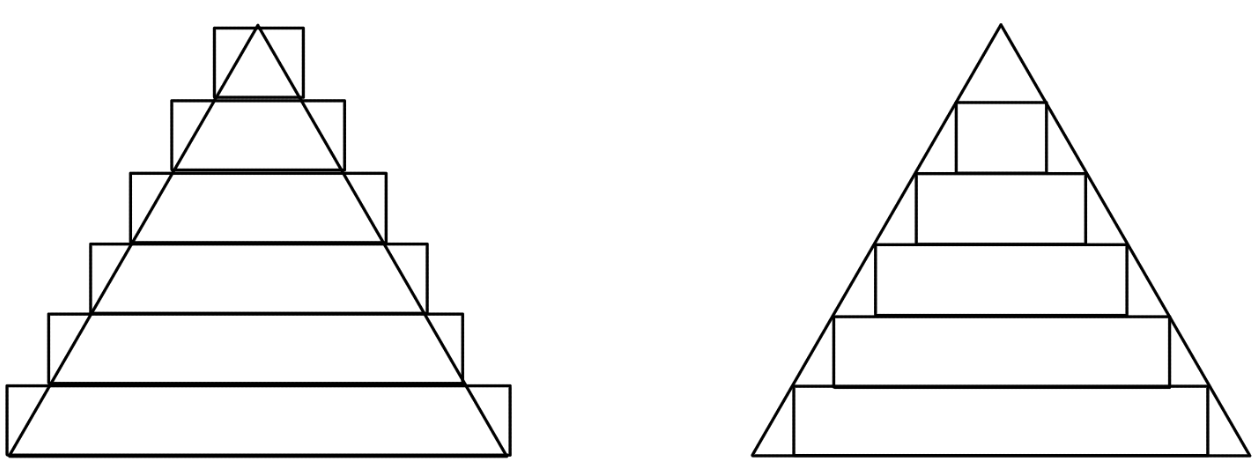
\includegraphics[width=0.5\textwidth, center]{piramide5.png}
  
        \[V_j = \Delta h \hspace{4.4pt}(l_j)^2\]

%Punto 2 del ejercicio 2
    \item Adapte el argumento que sugiere la siguiente figura (para el cálculo del volumen de un cono) al caso de la pirámide y aplíquelo para calcular los volúmenes $V_j$ de los prismas inscritos y circunscritos. 
 
        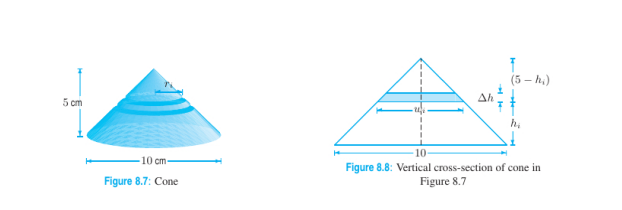
\includegraphics[width=0.5\textwidth, center]{cono.png} \\
        
        Teniendo el argumento, con la formula de calcular de un volumen j-ésimo y los siguientes datos:
    
            \begin{align*}
                V_j &= \Delta h(l_j)^2 \\
                \Delta h &= \frac{h}{50}\\
                P &= \left\{ \frac{0h}{50}, \frac{1h}{50}, \frac{2h}{50}, \frac{3h}{50}, \frac{4h}{50}, \dots,\frac{50h}{50} \right\}\\
                P &= \{ h_0, h_1, h_2, h_3, h_4, \dots, h_{50} \}\\
                h_j &= j \Delta h, \quad j = 1, 2, 3, 4, \dots, 50\\
            \end{align*}
            
        Primero tendríamos que obtener el valor de $l_j$. Por lo tanto, teniendo dos primas uno con base $l_0$ (siendo este el valor de la base de la pirámide) y otro con base $l_j$, si trazamos dos triángulos semejantes sobre las bases se puede obtener el valor de $ l_j$ de la siguiente forma:
        
        
        \begin{minipage}[H]{0.45\textwidth}
            \raggedleft
            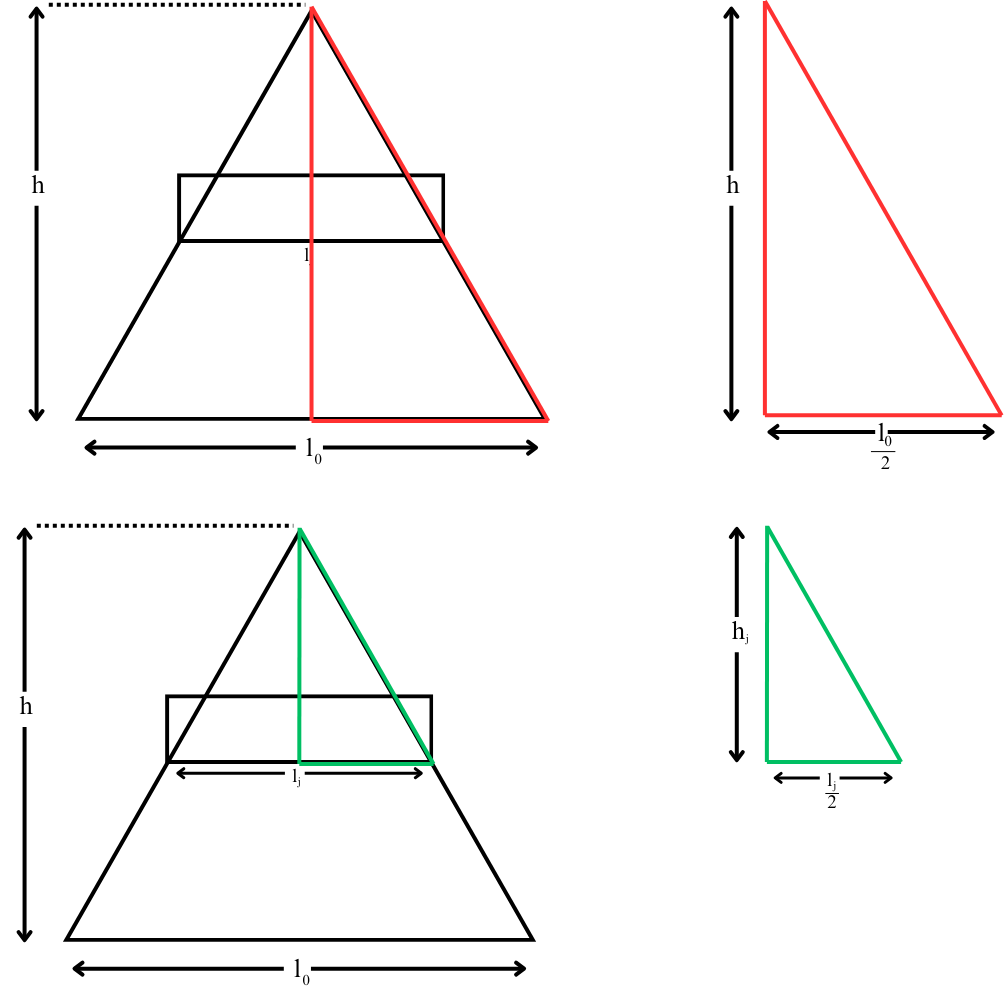
\includegraphics[width=\textwidth, center]{piramide2.png}
        \end{minipage}
        \hfill
        \begin{minipage}[H]{0.45\textwidth}
            \begin{align*}
                \frac{\frac{l_0}{2}}{h} &= \frac{\frac{l_j}{2}}{h - h_j}\\
                \frac{l_0}{2h} &= \frac{l_j}{2(h - h_j)}\\
                \frac{l_0 \cdot 2(h - h_j)}{2h} &= l_j\\
                \frac{l_0 \cdot (h - h_j)}{50h} &= l_j
            \end{align*}
        \end{minipage}
        
        Y sustituyendo el valor $l_j$ en la fórmula del volumen
    
        \begin{align*}
            V_j &= \Delta h \left( \frac{l_0 \cdot (h - h_j)}{h} \right)^2\\
            V_j &=   \frac{h \cdot l_0^2 \cdot (h - h_j)^2}{50 h^2} \\
            V_j &=   \frac{l_0^2 \cdot (h - h_j)^2}{50 h}\\
        \end{align*}
        Cabe señalar que tanto para los volúmenes inscritos y circunscritos la fórmula de $V_j$ funciona para ambos, solo que en la sumatoria de ambos, para el caso de los inscritos se empezará con un j=1 hasta 49.

%Punto 3 del ejercicio 2
    \item Sume los volúmenes que obtuvo en el inciso anterior y explique por qué el volumen de la pirámide del sol debe ser menor que la suma de los volúmenes de los prismas circunscritos y mayor que la suma de los volúmenes de los prismas inscritos.
     
    
        \begin{minipage}[H]{0.45\textwidth}
            \raggedleft
        \begin{align*}
            \sum_{j=0}^{50} \frac{l_0^2 \cdot (h - h_j)^2}{50h} &= \frac{l_0^2 \cdot }{50h}  \sum_{j=0}^{50}(h - h_j)\\
            &= \frac{l_0^2}{50h}  \sum_{j=0}^{50} \left(h -j \frac{h}{50} \right)^2\\
            &= \frac{l_0^2}{50h}  \sum_{j=0}^{50} \left(\frac{50j-jh}{50} \right)^2\\
            &= \frac{l_0^2}{50h}  \sum_{j=0}^{50} \frac{h^2}{50^2} \left(50-j \right)^2\\
            &= \frac{l_0^2 h^2}{50^3h}  \sum_{j=0}^{50} \left(50-j \right)^2\\
            &= \frac{l_0^2 h}{50^3}  \sum_{j=0}^{50} \left(50-j \right)^2\\
            &= \frac{l_0^2 h}{50^3} \left(\frac{50(50+1)(2(50)+1)}{6} \right) \\
            &= \frac{233.48^2 (71.17)}{125,000}(42,925)\\
            &= \frac {54,512.9104(71.17)(42,925)}{125,000}\\
            &= \frac {3,879,683.833168(42,925)}{125,000}\\
            &= \frac {166,535,428,538.7364}{125,000}\\
            &= 1,332,283.4283098912
        \end{align*}
        \end{minipage}
        \hfill
        \begin{minipage}[H]{0.45\textwidth}
            \raggedleft
            \begin{align*}
            \sum_{j=1}^{49} \frac{l_0^2 \cdot (h - h_j)^2}{50h} &= \frac{l_0^2 \cdot }{50h}  \sum_{j=0}^{50}(h - h_j)\\
            &= \frac{l_0^2}{50h}  \sum_{j=0}^{50} \left(h -j \frac{h}{50} \right)^2\\
            &= \frac{l_0^2}{50h}  \sum_{j=0}^{50} \left(\frac{50j-jh}{50} \right)^2\\
            &= \frac{l_0^2}{50h}  \sum_{j=0}^{50} \frac{h^2}{50^2} \left(50-j \right)^2\\
            &= \frac{l_0^2 h^2}{50^3h}  \sum_{j=0}^{50} \left(50-j \right)^2\\
            &= \frac{l_0^2 h}{50^3}  \sum_{j=0}^{50} \left(50-j \right)^2\\
            &= \frac{l_0^2 h}{50^3} \left(\frac{50(50+1)(2(50)+1)}{6} \right) \\
            &= \frac{233.48^2 (71.17)}{125,000}(42,925)\\
            &= \frac {54,512.9104(71.17)(42,925)}{125,000}\\
            &= \frac {3,879,683.833168(42,925)}{125,000}\\
            &= \frac {166,535,428,538.7364}{125,000}\\
            &= 1,332,283.4283098912
            \end{align*}    
        \end{minipage}
        
%Punto 4 del ejercicio 2
    \item ¿Qué espera que suceda con estas cotas al hacer los mismos cálculos para un número más y más grande?\\
     {\bf R:} El resultado convergerá al volumen real de la pirámide. 
   \end{enumerate}


\section{Series de potencias}

    {\bf Definición 1} \textit{Una serie de potencias en $q$ es una suma infinita de la forma:}\[\sum_{k=1}^{\infty} a_k q^k \tag{3}\]

    \textit{donde $q$ es un número real cualquiera y $a_k$ para $k = 1, 2, 3, \dots$ son coeficientes en $\mathbb{R}$. Se dice que la serie (3) converge a un valor $S \in \mathbb{R}$, si}\[S = \lim_{n \to \infty} \sum_{k=1}^{n} a_k q^k \tag{4}\]


    \textit{es decir, que basta tomar un valor de $n$ suficientemente grande para que $S_n$, la suma finita o suma parcial desde 1 hasta $n$, se acerque a $S$ tanto como se quiera.}

    \textit{Si $a_k = 1$ para toda $k$, la serie de potencias}
    \[\sum_{k=1}^{\infty} q^k \tag{5}\]
    \textit{se llama serie geométrica de razón $q$.}


    En clase se demostró la siguiente fórmula cerrada para las sumas parciales de la serie (5):

    \[S_n = \sum_{k=1}^{n} q^k = \frac{q (1 - q^n)}{1 - q} \tag{6}\]

    y, con base en (6), se resolvió la paradoja de Zenón relativa al viajero que va de Atenas a Esparta. De hecho, se explicó por qué:

    \[\sum_{k=1}^{\infty} \frac{1}{2^k} = 1.\]

    \begin{enumerate}
    
%Punto 1 del ejercicio 3
        \item Recupere los argumentos vertidos en clase para explicar por qué, si $q \geq 1$, la serie (5) no converge o, dicho de otro modo, diverge a $+\infty$.\\
            Para $q>1$ los términos $q^k$ crecen sin limite a medida que k aumenta.En este caso, la serie diverge porque los términos no se acercan a cero ni a ningún número en especifico y la suma es infinita.\\
Es decir, para $q>1$ tenemos que $q^k \rightarrow \infty$ cuando $k\rightarrow \infty$ por lo que $S_n = \sum_{k=1}^{n} q^k \rightarrow \infty$
    

%Punto 2 del ejercicio 3
        \item Suponga ahora que $q \leq 0$. ¿Para qué valores de $q$ converge la serie (5)? En su respuesta, considere los siguientes casos:(a) $-1 < q \leq 0$, (b) $q = -1$ y (c)$q < -1$. Para tener una idea, es conveniente experimentar numéricamente en una hoja de cálculo (como se hizo en clase) con distintos valores de $q$ y, luego, buscar un argumento que explique el comportamiento general.\\
     \\ Para analizar mejor la serie obtendremos la formula de la suma infinita de la serie para apoyarnos a calcular cuando converge \\ 
    Escribimos la serie 
    \begin{eqnarray*}
        S=  q + q^2 + q^3+ q^4+ q^5+ ...
    \end{eqnarray*}
    
    Y multiplicamos cada termino de la serie por q
    \begin{eqnarray*}
           q S= q^2 + q^3+ q^4+ q^5+ q^6 ...
    \end{eqnarray*}
    Restamos la serie multiplicada de la original\\
    \begin{eqnarray*}
   S- qS =  (q + q^2 + q^3+ q^4+ q^5+ ...)& -  (q^2 + q^3+ q^4+ q^5+ q^6 ...)   \\
         S- qS= q \\
       S(1-q)=q \\
       S= \frac{q}{1-q}         
    \end{eqnarray*}\\

Así obtenemos la formula para obtener para las suma infinita de la serie.\\
 Observando la serie vemos que si $|q|<1$ va a converger y va a converger a la suma calculada anteriormente, ya que los  términos $q^k$  se acercan a cero conforme a k aumenta.\\
Observemos este caso y los otros dos:

\begin{itemize}
    \item $-1< q \leq 0$ \\
    Realizamos una tabla para analizar como se comporta la suma cuando q se encuentra en este rango:
          \begin{table} [h]
            \begin{center}
                \begin{tabular}{| c | c | c |}\\ \hline
                    q &     Serie & Suma de la serie  \\ \hline
                    -0.999 &  $(-.999)^1 + (-.999)^2 + (-.999)^3 +\ldots+(-.999)^n$ &  -0.4997   \\ \hline
                    -0.99 &  $(-.99)^1 + (-.99)^2 + (-.99)^3 +\ldots+(-.99)^n$ &    -0.4974\\ \hline
                    -0.9& $(-.9)^1 + (-.9)^2 + (-.9)^3 +\ldots+(-.9)^n$ &  -0.4736    \\ \hline
                    -0.1 & $(-.1)^1 + (-.1)^2 + (-.1)^3 +\ldots+(-.1)^n$  &  -0.0909  \\ \hline
                    -0.01& $(-.01)^1 + (-.01)^2 + (-.01)^3 +\ldots+(-.01)^n$ &   -0.0099 \\ \hline
                    -0.001& $(-.001)^1 + (-.001)^2 + (-.001)^3 +\ldots+(-.001)^n$ &   -0.0009  \\ \hline
                    -0.0001 & $(-.0001)^1 + (-.0001)^2 + (-.0001)^3 +\ldots+(-.0001)^n$ &  -0.00009   \\ \hline
                    0 & $(0)^1 + (0)^2 + (0)^3 +\ldots+(0)^n$& 0    \\ \hline
                \end{tabular}

                \label{tab:datos}
            \end{center}
          \end{table}
Observamos que en cada valor dentro del rango $-1<q\leq 0$ conforme k aumenta el valor de $q^k$ se acerca más a cero y la serie converge.

    
    


    
    \item $q=-1$\\
    En la tabla observamos como se comporta la serie con q=1, es decir como se comporta $\sum_{k=1}^{n} (-1)^k $
    \begin{table} [H]
    \centering
\begin{tabular}{| c | c | c |}
\hline
q &     Serie & Suma de la serie  \\ \hline
 -1 & $(-1)^1 + (-1)^2 + (-1)^3 +\ldots+(-1)^n$ = $-1+1-1+1-1+1...$ & Oscila entre 0 y -1  \\ \hline
\end{tabular}
\label{tab:datos}
\end{table}
La serie en este caso se convierte en una serie alternante que no converge. No converge a un limite finito, porque los términos no se estabilizan en torno a un valor único. En cambio la suma oscila entre 0 y -1.


    \item $q<-1$
\\
Para este caso tomamos diferentes valores negativos de q para observar el comportamiento de la serie:
   \begin{table} [H]
    \centering   
\begin{tabular}{| c | c | c |}
\hline
q &     Serie & Suma de la serie  \\ \hline
-2 &  $(-2)^1 + (-2)^2 +\ldots+(-2)^n$= $(-2) +4 + (-8) +(16)+ ...$ & \\ 
 -3 &  $(-3)^1 + (-3)^2 +\ldots+(-3)^n$=    $(-3) +9 + (-27) +(81)+ ...$ &\\ 
 -4& $(-4)^1 + (-4)^2 +\ldots+(-4)^n =(-4) +16 + (-64) +(256)+ ...$  &  No tienen     \\
 -5 & $(-5)^1 + (-5)^2 +\ldots+(-5)^n$ = $(-5) +25 + (-125) +(625)+ ...$ &  suma finita   \\ 
-10 &$(-10)^1 + (-10)^2 +\ldots+(-10)^n$ =$(-10) +100 + (-1000)+ ...$  &    \\ \hline
\end{tabular}

\label{tab:datos}

\end{table}
Observamos que cuando $q<-1$ la serie $\sum_{k=1}^{n} (q)^k $ diverge. Los términos de la serie alternan el signo y crecen en magnitud, lo que significa que no se acercan a ningún valor en especifico y la serie no tiene una suma finita.
    
\end{itemize}
\end{enumerate}
 \section{\large Un balón de futbol americano} 
 En este ejercicio se trata de calcular aproximadamente el volumen \( V \) de un balón de fútbol americano profesional suponiendo que su superficie se genera rotando, alrededor del eje horizontal, una curva \( y = y(x) \) que satisface que la longitud del eje entre las dos puntas del balón es de 28 cm y la circunferencia de la máxima sección circular transversal al eje mide 53 cm (véase la siguiente figura).\\
    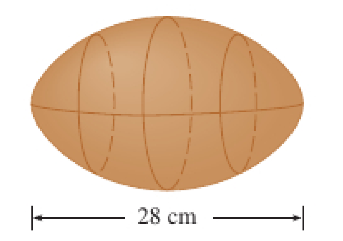
\includegraphics[width=0.5\textwidth, center]{balon.png}


Rebane la mitad derecha del balón en 10 cilindros de grosor \( \Delta x = 1.4 \) cm, de manera que las rebanadas intersecten el eje \( x \) en los valores de la siguiente partición del intervalo \([0, 14]\):

\[
P = \{x_k \mid x_k = k \Delta x \text{ para } k = 0, \ldots, 10\}
\]

es decir que:

\[
x_0 = 0, \quad x_1 = 1.4, \quad x_2 = 2.8, \quad x_3 = 4.2, \quad \ldots, \quad x_9 = 12.6, \quad x_{10} = 14.
\]

Entonces, si \( V_k \) es el volumen del \( k \)-ésimo cilindro,

\[
V \approx \sum_{k=1}^{10} V_k
\]
\begin{itemize}
\item Suponga que la curva \( y = y(x) \) es un arco de parábola cuyo vértice coincide con el punto más alto de la máxima sección transversal perpendicular al eje \( x \) y que intersecta al eje horizontal en los puntos \((-14, 0)\) y \((14, 0)\). Entonces:

\begin{enumerate}
    \item Muestre que la parábola es, aproximadamente, la gráfica de la función

\[
y(x) = -0.043 x^2 + 8.4352
\]

definida para \(-14 \leq x \leq 14\).\\
{\bf R:} Se tiene que la función de una parábola está denotada por:

\[ y(x)=ax^2+bx+c\]

Sabemos que la punto del vértice de la parábola con respecto al origen es $(0, \frac{53}{2\pi)}$ ya que la circunferencia del circulo situado a la mitad del  balón es 53 que se obtiene de la formula de  $P = 2\pi r$. Si sustituimos este valor en la fórmula de la parábola obtenemos $c$:

        \begin{align*}
            y(0)= \frac{53}{2\pi} &= a(0)^2+b(0)+c\\
            \frac{53}{2\pi} &= c
        \end{align*}
  
        Si ahora usamos los puntos donde la parábola toca al eje $x$ tendríamos a $a$ y $b$:
        
       \begin{align*}
            y(14)=0&= a(14)^2+b(14)+c &\quad y(-14)=0&= a(-14)^2+b(14)+c\\
             &= a(14)^2+b(14)+c &\quad &= a(-14)^2+b(-14)+c\\
            &= 196a+14b+c &\quad &= 196a-14b+c\\ 
        \end{align*}
            Si sumamos ambos resultados tenemos:\\
            
            \[
            \begin{array}{c}
            196a+14b+c\\
            196a-14b+c\\
            \hline
            392a +2c = 0\\
            \end{array}
            \]
        
        Si despejamos a $a$.
            
        \[a=- \frac{c}{196}\]
        Si queremos obtener a $b$, solo haría falta cambiar los signos a un valor y volverlos a sumar, y después despejar a $b$
        \[
        \begin{array}{c}
            196a+14b+c \\
            -196a+14b-c\\\hline
            28b = 0\\
            b=0
        \end{array}
        \]
    Teniendo ya las literales solo hace falta sustituirlas y desarrollar la ecuación:
\begin{align*}
   y(x)&=- \frac{\frac{53}{2\pi}}{196}x^2+\frac{53}{2\pi}\\ 
   y(x)&=- \frac{53}{392\pi}x^2+8.4352\\
   y(x)&=- -0.043 x^2+8.4352\\
\end{align*}



\item Muestre que la aproximación del volumen con los 10 cilindros circunscritos de grosor \( \Delta x = 1.4 \) cm y radios \( y(x_k) \) cm para \( k = 0, 1, 2, \ldots, 9 \) es:

\[
V \approx 2 \times 1825.5143 = 3651.0286 \text{ cm}^3
\]

{\bf R:} 
\begin{table}{H}
    \centering
\begin{tabular}{|c|c|c|c|}\hline
    $V_k$ &Radio{cm} & Área [$cm^2$] & Volumen[$cm^3$]\\ }\hline
     0 & 8.4352 & 233.533 & 312.946 \\
     1 & 8.375 & 220.353 & 308.495 \\
     2 & 8.3148 & 217.1973 & 304.076\\
     3 & 8.2546 & 214.0636 & 299.6891\\
     4 & 8.1944 & 210.9527 & 295.333\\
     5 & 8.1342 & 207.8646 & 291.0104\\
     6 & 8.074 & 204.7992 & 286.7189\\
     7 & 8.0138 & 201.756 & 282.4593\\
     8 & 7.9536 & 198.7368 & 278.2315\\
     9 & 7.8934 & 195.7397 & 274.0357\\\hline
      \multicolumn{2}{|c|}{}Sumatoria & 2932.9968 cm$^3$\\\hline
\end{tabular}
\label{tab:CilCirPar}
\end{table}
\item Muestre que la aproximación del volumen con los 10 cilindros inscritos de grosor \( \Delta x = 1.4 \) cm y radios \( y(x_k) \) cm para \( k = 1, 2, \ldots, 10 \) es:
\end{enumerate}
\[
V \approx 2 \times 1512.5672 = 3025.1344 \text{ cm}^3
\]

\item Suponga ahora que la curva \( y = y(x) \) es la mitad superior de una elipse con centro en el origen, semieje horizontal \( a = 14 \) cm (sobre el eje \( x \)) y semieje vertical \( b = \frac{53}{2\pi} \approx 8.4352 \) cm (sobre el eje \( y \)).

\item Muestre que el arco de elipse es, aproximadamente, la gráfica de la función

\[
y(x) = 0.6025 \sqrt{196 - x^2}
\]

definida para \(-14 \leq x \leq 14\).

\item Muestre que la aproximación del volumen con los 10 cilindros circunscritos de grosor \( \Delta x = 1.4 \) cm y radios \( y(x_k) \) cm para \( k = 0, 1, 2, \ldots, 9 \) es:

\[
V \approx 2 \times 2237.4593 = 4474.9186 \text{ cm}^3
\]

\item Muestre que la aproximación del volumen con los 10 cilindros inscritos de grosor \( \Delta x = 1.4 \) cm y radios \( y(x_k) \) cm para \( k = 1, 2, \ldots, 10 \) es:

\[
V \approx 2 \times 1924.5279 = 3849.0558 \text{ cm}^3
\]

    \end{itemize}
\end{document}
